\chapter{Introducing ANTLR}
If the task is to implement a parser, it is best to use one of the tools that is available for this purpose.
The wikipedia page 
\\[0.2cm]
\hspace*{1.3cm}
\href{https://en.wikipedia.org/wiki/Comparison_of_parser_generators}{Comparison of parser generators}
\\[0.2cm]
shows the large number of parser generators that are available.
In my opinion, the parser generator that is both most mature and most powerful is
\textsc{Antlr} \index{\textsc{Antlr}} \cite{parr:2012,parr:2014}.  The name is short for 
\emph{\underline{an}other \underline{t}ool for \underline{l}anguage \underline{r}ecognition}\footnote{
  The name \textsc{Antlr} can also be interpreted as an acronym for \underline{ant}i \underline{LR},
  where ``LR'' is short for \emph{LR} parser.  LR parsers are a kind of \emph{bottom-up parsers}.  We will discuss these
  parsers later in chapter \ref{chapter:bottom-up}.
}.
\textsc{Antlr} can be downloaded at 
\\[0.2cm]
\hspace*{1.3cm}
\href{http://www.antlr.org}{\texttt{http://www.antlr.org}}.
\\[0.2cm]
In this lecture we will use \textsc{Antlr} version 4.8.  The tool \textsc{Antlr} is written in \textsl{Java}
but can be used to generate parsers for the programming languages \textsl{Java}, \texttt{C++}, \texttt{C\#},
\textsl{Python}, \textsl{JavaScript}, \textsl{Go}, and \textsl{Swift}.
We will introduce \textsc{Antlr} via some examples that demonstrate the most important features of this tool.
For lack of time we will only discuss the most important features of \textsc{Antlr}.  For a discussion of all
the features offered by \textsc{Antlr} I recommend the book ``The Definitive \textsc{Antlr} Reference'' by
Terrence Parr \cite{parr:2012}.

\section{A Parser for Arithmetic Expressions}
We start with a parser for arithmetic expressions.  The structure of arithmetic expressions can be described by
the grammar that is shown in Figure \ref{fig:Expr} on page \pageref{fig:Expr}.
If we use \textsc{Antlr} we can implement this grammar as shown in Figure \ref{fig:Expr.g4}.  
We discuss the implementation line by line.

\begin{figure}[!ht]
\centering
\begin{minted}[ frame         = lines, 
                framesep      = 0.3cm, 
                numbers       = left,
                numbersep     = -0.2cm,
                bgcolor       = sepia,
                xleftmargin   = 0.8cm,
                xrightmargin  = 0.8cm,
              ]{antlr}
    grammar Expr;
    
    start   : expr
            ;
    
    expr    : expr '+' product 
            | expr '-' product
            | product        
            ;
    
    product : product '*' factor 
            | product '/' factor 
            | factor
            ;
    
    factor  : '(' expr ')'
            | NUMBER
            ;
    
    NUMBER  : '0'|[1-9][0-9]*;
    WS      : [ \t\n\r] -> skip;
\end{minted}
\vspace*{-0.3cm}
\caption{\textsc{Antlr}-Spezifikation eines Parsers f\"ur arithmetische Ausdr\"ucke.}
\label{fig:Expr.g4}
\end{figure}


\begin{enumerate}
\item In line 1 the keyword \texttt{grammar} specifies the name of the grammar.
      In this case the grammar is called \texttt{Expr}.  The name of the file that contains this grammar is
      created by appending the file extension  ``\texttt{.g4}''.  Therefore this grammar 
      has to be stored in a file with the name ``\texttt{Expr.g4}''.
\item Line 3 gives the production for the non-terminal \textsl{start}.  In the last chapter we had used the
      notation
      \hspace*{1.3cm}
      $\textsl{start} \rightarrow \textsl{expr}$
      \\[0.2cm]
      instead.  With \textsc{Antlr} the left and right part of a production are separated by a colon.
      \textsc{Antlr} terminates every production with the character ``\texttt{;}
\item Line 6--9 give the productions for the non-terminal \textsl{expr}.  Note that we have to enclose the 
      terminals ``\texttt{+}'' and ``\texttt{-}'' in single quotes.  The different rules for the non-terminal
      \texttt{expr} are separated by the character ``\texttt{|}''.
\item Similarly, the lines 11--14 and 16--18 show the productions for the non-terminals \textsl{product} and
      \textsl{factor}.   
\item With \textsc{Antlr} the grammar and the specification of the tokens can be given in the same file.
      In order to be able to distinguish terminals and non-terminals, terminals have to begin with an upper case 
      letter,\footnote
      {It is a convention that the names of non-terminals consist of only upper case letters, but this is not required.}
      while non-terminals start with a lower case letter.   Therefore, ``\texttt{NUMBER}'' is the name
      of a terminal.
\item In line 20 the lexical specification of the non-terminal \texttt{NUMBER} is given
      by a regular expression.  The regular expression
      \\[0.2cm]
      \hspace*{1.3cm}
      \texttt{'0'|[1-9][0-9]*;}
      \\[0.2cm]
      describes a sequence of digits.  This sequence can only start with the digit
      ``\texttt{0}'' when ``\texttt{0}'' not followed by any other digit.

      Notice that we have to enclose the first occurrence of ``\texttt{0}'' in single quotes.
      On the other hand, we must not put the digits occurring in the square brackets ``\texttt{[}'' 
      and ``\texttt{]}'' in quotes, since these occur inside \blue{range} and characters inside a range
      must never be quoted.
\item Line 21 defines the terminal \texttt{WS}, where the name is short for \emph{white space}. This terminal
      specifies a single character that is either a blank, a tabulator, a line break, or a carriage return.
      The lexical specification of the terminal \texttt{WS} is followed by the operator ``\texttt{->}'' 
      which in turn is followed by a \blue{semantic action}.
      The semantic action ``\texttt{skip}'', which is executed once a white space character has be recognized, 
      simply discards the white space character.  Therefore we cannot use the terminal \texttt{WS} in our
      grammar rules.  Therefore, the net effect of line 21 is to discard all white space characters.

      In most programming languages\footnote{
        Unfortunately, \textsl{Python} is an exception to this rule.  Therefore, parsing
        \textsl{Python} is considerably harder than parsing languages like \texttt{C} or \textsl{Java}.
      }, white space has no purpose other than that of separating  tokens.  
      Therefore, most \textsc{Antlr} parsers will have a scanner rule that is similar to
      the rule shown in line 21. 
\end{enumerate}
To conclude, the lines 3--18 specify the grammar, while the line 20--21 specify the 
lexical structure.  If the grammar that is shown in Figure \ref{fig:Expr.g4} is stored in the file
\href{https://github.com/karlstroetmann/Formal-Languages/blob/master/ANTLR4-Python/PureExprParser/Expr.g4}{\texttt{Expr.g4}} 
we can generate a parser by using the following command:
\\[0.2cm]
\hspace*{1.3cm}
\texttt{java -jar /usr/local/lib/antlr-4.8-complete.jar -Dlanguage=Python3 Expr.g4}
\\[0.2cm]
Of course, this only works if the file \texttt{antlr-4.8-complete.jar} is stored in the directory
\texttt{/usr/local/lib/}.  Among others, \texttt{Antlr} will then generate the following files:
\begin{enumerate}
\item \texttt{ExprParser.py}

      This file contains the parser.
\item \texttt{ExprLexer.java}

      This is the scanner.
\item \textsc{Antlr} generates some more files.  However, these are not relevant for us.
\end{enumerate}

In order to run the parser we need a driver program.  Figure \ref{fig:PureParser.ipynb} shows such a program.

\begin{figure}[!ht]
\centering
\begin{Verbatim}[ frame         = lines, 
                  framesep      = 0.3cm, 
                  labelposition = bottomline,
                  numbers       = left,
                  numbersep     = -0.2cm,
                  xleftmargin   = 0.8cm,
                  xrightmargin  = 0.8cm,
                ]
    from ExprLexer  import ExprLexer
    from ExprParser import ExprParser
    
    import antlr4
    
    def parse_string(string): 
        inputStream = antlr4.InputStream(string)
        lexer       = ExprLexer(inputStream)
        stream      = antlr4.CommonTokenStream(lexer)
        parser      = ExprParser(stream)
        parser.start()
\end{Verbatim}
\vspace*{-0.3cm}
\caption{Driver program for the parser generated by \textsc{Antlr}.}
\label{fig:PureParser.ipynb}
\end{figure}

\begin{enumerate}
\item In Line 1 and 2 we import the scanner and the parser that has been generated by \textsc{Antlr}.
\item Line 7 transforms the input from a string into an object of class \texttt{InputStream}.
      This object is then used to create the scanner \texttt{lexer}.
\item Using this scanner we create an object of class \texttt{CommonTokenStream}.
      This object is then fed into the parser in line 10.
\item The parser is called in line 11.  In order to call the parser we have to invoke the method 
      \texttt{start}.  Here \texttt{start} is the name of the non-terminal that is to be recognized
\end{enumerate}
If we want to test our parser we use the command:
\\[0.2cm]
\hspace*{1.3cm}
\texttt{parse\_string(\symbol{34}1 + 2 * 3 - 4\symbol{34})}
\\[0.2cm]
This will run without errors, showing that the input adheres to the specification of the grammar.
If we want to see the parse tree instead, we have to use the \texttt{TestRig} provided by \textsc{Antlr}.
In order to use the \texttt{TestRig}, we first have to create the some \textsl{Java} files using the command
\\[0.2cm]
\hspace*{1.3cm}
\texttt{java -jar /usr/local/lib/antlr-4.8-complete.jar -Dlanguage=Java Expr.g4}
\\[0.2cm]
The generated \textsl{Java} files have to be compiled with the following command:
\\[0.2cm]
\hspace*{1.3cm}
\texttt{javac -cp .:/usr/local/lib/antlr-4.8-complete.jar *.java}
\\[0.2cm]
After that we can generate a parse tree using the command
\\[0.2cm]
\hspace*{0.3cm}
\texttt{java -cp .:/usr/local/lib/antlr-4.8-complete.jar org.antlr.v4.gui.TestRig Expr start -gui}
\\[0.2cm]
This command will open a tree viewer that shows the parse tree of any input we have typed in response to this command.
For the input string ``\texttt{1 + 2 * 3 - 4}''  this tree looks as as shown in Figure \ref{fig:expr.eps}.

\begin{figure}[!ht]
  \centering
      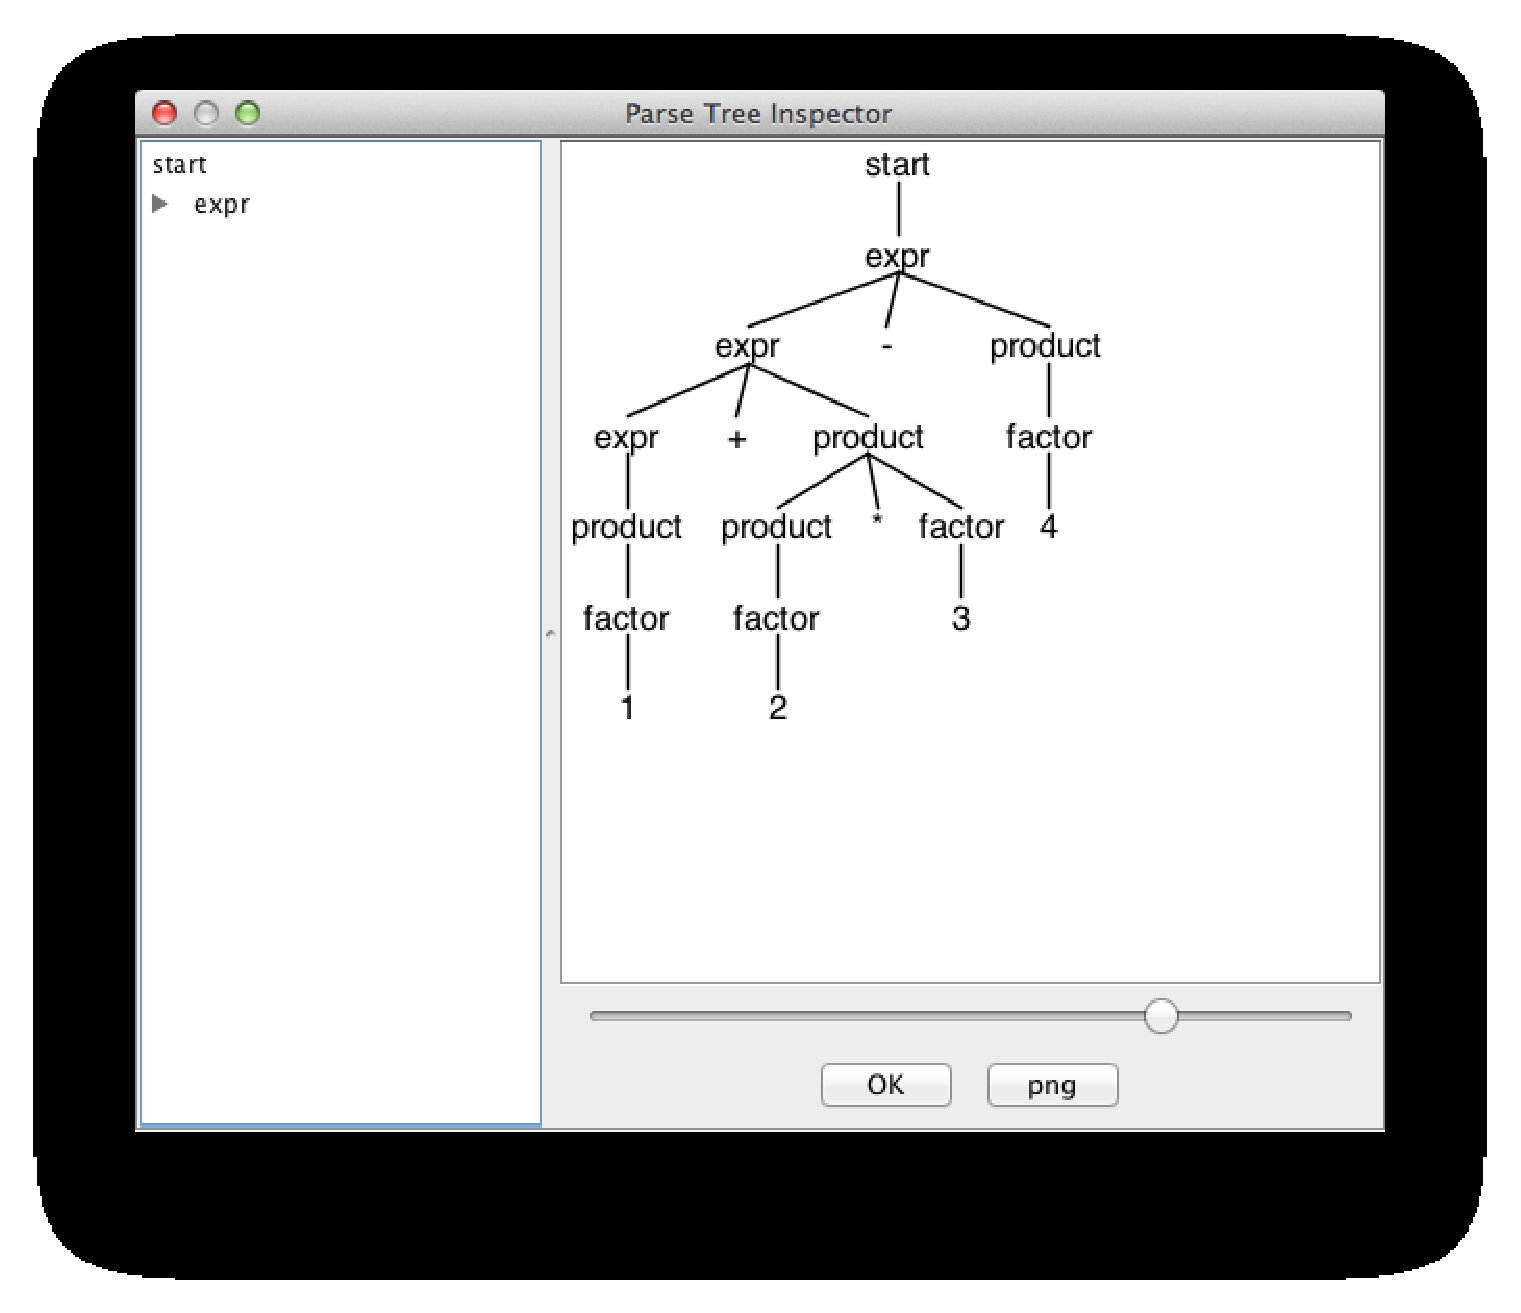
\epsfig{file=Abbildungen/expr.eps, scale=0.7}
   \caption{Parse tree for the string ``\texttt{1 + 2 * 3 - 4}''.}
  \label{fig:expr.eps}
\end{figure}



\section{Evaluation of Arithmetical Expressions}
The last example isn't very exciting as the arithmetical expressions that the parser has read are not
evaluated.  In this section we show how arithmetical expressions can be evaluated using \textsc{Antlr}
generated parsers.  We proceed in two steps:
\begin{enumerate}
\item Firstly, we present a grammar for small symbolic calculator.
\item Secondly, we show how this grammar can be extended with actions so that the expressions can be evaluated.
\end{enumerate}

gespeichert werden k\"onnen.  Wir gehen dabei in zwei Schritten vor und pr\"asentieren
zun\"achst eine reine Grammatik in \textsc{Antlr}-Notation.  Anschlie{\ss}end erweitern wir diese
mit Aktionen, in denen die Ausdr\"ucke ausgewertet werden k\"onnen.
Abbildung \ref{fig:Program.g4} zeigt diese Grammatik.  Gegen\"uber der vorher gezeigten
Grammatik f\"ur arithmetische Ausdr\"ucke gibt es die folgenden \"Anderungen:

\begin{figure}[!ht]
\centering
\begin{Verbatim}[ frame         = lines, 
                  framesep      = 0.3cm, 
                  labelposition = bottomline,
                  numbers       = left,
                  numbersep     = -0.2cm,
                  xleftmargin   = 0.8cm,
                  xrightmargin  = 0.8cm,
                ]
    grammar Program;
    
    program : stmnt+ ;
    
    stmnt   : ID ':=' expr ';'
            | expr ';'
            ;    
    
    expr    : expr ('+'|'-') product
            | product
            ;
    
    product : product ('*'|'/') factor
            | factor
            ;
    
    factor  : '(' expr ')'
            | ID
            | INT
            ;
    
    ID : [a-zA-Z][a-zA-Z0-9]*;
    INT: '0'|[1-9][0-9]*;
    WS : [ \v\t\n\r] -> skip; 
\end{Verbatim}
\vspace*{-0.3cm}
\caption{Eine Grammatik f\"ur die Auswertung von Ausdr\"ucken.}
\label{fig:Program.g4}
\end{figure}


\begin{enumerate}
\item Das Start-Symbol ist jetzt \texttt{program}.  Es steht f\"ur eine Liste
      von Zuweisungen der folgenden Form:
      \\[0.2cm]
      \hspace*{1.3cm}
      $\textsl{var} \;\mathtt{:=}\; \textsl{expr}\mathtt{;}$
      \\[0.2cm]
      Hier ist \texttt{var} der Name einer Variablen und \textsl{expr} ist ein
      arithmetischer Ausdruck.
\item \texttt{stmnt} bezeichnet eine Zuweisung oder einen einzelnen Ausdruck.
\item Wir haben die Regeln f\"ur die syntaktischen Variablen \textsl{expr} und \textsl{product}
      vereinfacht, indem wir jeweils die beiden Operatoren ``\texttt{+}'' und ``\texttt{-}'' bzw.
      \squoted{*} und \squoted{/} zusammengefasst haben.
      Da \textsc{Antlr} \textsc{Ebnf}-Grammatiken unterst\"utzt, k\"onnen wir f\"ur \textsl{expr}
      beispielsweise die Regel
      \\[0.2cm]
      \hspace*{1.3cm}
      \texttt{expr : expr ('+'|'-') product | product ;}
      \\[0.2cm]
      verwenden.  Die Grammatik-Regel f\"ur \textsl{product} haben wir in \"ahnlicher Weise
      ge\"andert.
\item Das Terminal \texttt{ID} bezeichnet den Namen einer Variablen.  Ein solcher Name
      besteht aus einer beliebigen Folge von Buchstaben und Ziffern, die mit einem Buchstaben 
      beginnen muss.
\end{enumerate}
Mit diesem Parser k\"onnen wir jetzt zum Beispiel die folgende Eingabe parsen:
\begin{verbatim}
    x = 2 * 3; y = 4 * 5; z = x * x + y * y; 
    z / 3;
\end{verbatim}
Wir wollen nun einen ganz einfachen Interpreter entwickeln, der eine Folge von solchen
Zuweisungen auswertet und die bei der Auswertung berechneten Zwischen-Ergebnisse
in Variablen abspeichert, auf die in folgenden Ausdr\"ucken Bezug genommen werden kann.
Weiterhin soll jeder Ausdruck, der keiner Variablen zugewiesen wird, ausgewertet und
ausgegeben werden.  Abbildung \ref{fig:Program.g4-2} zeigt die Realisierung eines solchen
Interpreters mit \textsc{Antlr}.

\begin{figure}[!ht]
\centering
\begin{Verbatim}[ frame         = lines, 
                  framesep      = 0.3cm, 
                  labelposition = bottomline,
                  numbers       = left,
                  numbersep     = -0.2cm,
                  xleftmargin   = 0.3cm,
                  xrightmargin  = 0.3cm,
                ]
    grammar Program;
     
    @header {
        import java.util.TreeMap;
    }
    
    @members {
        TreeMap<String, Integer> varTable = new TreeMap<String, Integer>();
    }
    
    program : stmnt+ ;
    
    stmnt : ID ':=' expr ';' { varTable.put($ID.text, $expr.result); }
          |         expr ';' { System.out.println($expr.result);     }
          ;    
    
    expr returns [int result]
        : e = expr { $result = $e.result; }
          (   '+' p = product { $result += $p.result; }
            | '-' p = product { $result -= $p.result; }
          )
        | p = product { $result = $p.result; }
        ;
    
    product returns [int result]
        : p = product { $result = $p.result; }
          (
              '*' f = factor { $result *= $f.result; }
            | '/' f = factor { $result /= $f.result; }
          )
        | f = factor { $result = $f.result; }
        ;
    
    factor returns [int result]
        : '(' expr ')' { $result = $expr.result;           }
        | ID           { $result = varTable.get($ID.text); }
        | INT          { $result = new Integer($INT.text); }
        ;
    
    ID : [a-zA-Z][a-zA-Z0-9]*;
    INT: '0'|[1-9][0-9]*;
    WS : [ \v\t\n\r] -> skip; 
\end{Verbatim} 
%\$
\vspace*{-0.3cm}
\caption{Ein Interpreter zur Auswertung von Ausdr\"ucken.}
\label{fig:Program.g4-2}
\end{figure}

\begin{enumerate}
\item Da wir die Werte der einzelnen Variablen in einer Tabelle abspeichern m\"ussen,
      importieren wir in den Zeilen 3 -- 5 die Klasse \texttt{java.util.TreeMap}, denn
      diese Klasse implementiert Tabellen effizient als bin\"are B\"aume.

      Allgemein setzt \textsc{Antlr} all den Code, der durch das Schl\"usselwort
      ``\texttt{@header}'' spezifiert wird, an den Anfang der erstellten Parser-Datei.
\item In den Zeilen 7 -- 9 definieren wir zus\"atzliche Member-Variablen f\"ur die erzeugte
      Klasse \texttt{ProgramParser}.  In unserem Fall definieren wir hier die Tabelle, die
      sp\"ater die Werte der Variablen enth\"alt, als Abbildung, die Strings ganze Zahlen zuordnet.

      Allgemein setzt \textsc{Antlr} all den Code, der durch das Schl\"usselwort
      ``\texttt{@members}'' spezifiert wird, an den Anfang der erstellten Parser-Klasse.
      Dieses Feature kann sowohl zur Definition von zus\"atzlichen Klassen-Variablen als auch
      von Methoden verwendet werden.
      
      Wir reichern nun die Grammatik-Regeln mit Aktionen an, die durchgef\"uhrt werden, wenn
      der Parser die entsprechende Grammatik-Regel anwendet.  Die Aktionen werden von der
      eigentlichen Grammatik-Regel, f\"ur die sie angewendet werden sollen, dadurch
      abgesetzt, dass sie in den geschweiften Klammern ``\texttt{\{}'' und ``\texttt{\}}''
      eingefasst werden.
\item Wird vom Parser in Zeile 13 eine Zuweisung der Form $\textsl{var} \;\mathtt{:=}\; \textsl{expr}$
      erkannt,  
      so soll der Wert des Ausdrucks \textsl{expr} berechnet und das Ergebnis in der
      Tabelle \texttt{varTable} unter dem Namen \textsl{var} eingetragen werden.
      In der Grammatik-Regel
      \\[0.2cm]
      \hspace*{1.3cm}
      \textsl{stmnt} $\rightarrow$ \texttt{ID} ':=' \textsl{expr} ';'
      \\[0.2cm]
      haben wir einerseits das Token \texttt{ID}, auf dessen Namen wir mit \texttt{\symbol{36}ID.text}
      zugreifen k\"onnen, andererseits haben wir die syntaktische Variable \textsl{expr}.
      Wir werden sp\"ater dieser syntaktischen Variable die \textsl{Java}-Variable
      \texttt{result} als Ergebnis-Variable zuordnen, die den zugeh\"origen Wert enth\"alt.  
      Dann k\"onnen wir mit
      \texttt{\symbol{36}expr.result} auf diesen Wert zugreifen.

      In Zeile 14 haben wir einen einzelnen arithmetischen Ausdruck, den wir auswerten und ausgeben.
\item In Zeile 17 definieren wir mit der Zeile
      \\[0.2cm]
      \hspace*{1.3cm}
      \texttt{expr returns [int result]}
      \\[0.2cm]
      dass die Methode, die eine \textsl{expr} parst, als Ergebnis ein \texttt{int} zur\"uck
      gibt und dass dieses in der Variable mit dem Namen \texttt{result} abgespeichert wird.
\item In der Grammatik-Regel
      \\[0.2cm]
      \hspace*{1.3cm}
      \texttt{expr : expr ('+'|'-') product | product ;}
      \\[0.2cm]
      haben wir in Zeile 18 -- 20 den verschiedenen Auftreten der syntaktischen Variablen
      \texttt{expr} und \texttt{product} die Namen $e$ und $p$ zugeordnet, auf die wir dann in den
      Aktionen zugreifen k\"onnen.  In den Aktionen muss diesen Variablen allerdings ein Dollar-Zeichen
      vorgestellt werden.

      Die Aktionen selber bestehen nun darin, dass wir der Variablen \texttt{result}
      das Ergebnis der jeweiligen Berechnung zuweisen.
\item In den Zeilen 36 und 37 greifen wir auf die Strings, die den Token
      \texttt{ID} und \texttt{INT} entsprechen, mit Hilfe der f\"ur Token vordefinierten
      Variable \texttt{text} zur\"uck.  Beachten Sie, dass wir in Zeile 36 den Wert, der zu einer
      Variablen in der Tabelle \texttt{varTable} gespeichert ist, auslesen und als Ergebnis zur\"uck
      geben. 
\end{enumerate}

\section{Erzeugung abstrakter Syntax-B\"aume}
Bei der Auswertung arithmetischer Ausdr\"ucke im letzten Abschnitt hatten wir Gl\"uck
und konnten das Ergebnis eines Ausdrucks unmittelbar mit Hilfe von semantischen Aktionen
berechnen.  Bei komplexeren Problemen ist es in der Regel erforderlich, zun\"achst einen
abstrakten Syntax-Baum zu erzeugen.  Die eigentliche Berechnung findet dann erst nach dem
Parsen auf dem Syntax-Baum statt.  Wir wollen dieses Verfahren an einem Beispiel
demonstrieren.  Bei dem Beispiel geht es wieder um die symbolische Differentiation
arithmetischer Ausdr\"ucke.  Ist beispielsweise der arithmetische Ausdruck 
\[ x \cdot \ln(x) \]
gegeben, so findet sich f\"ur die Ableitung dieses Ausdrucks nach der Variable $x$ mit Hilfe
der Produkt-Regel das
Ergebnis 
\[ 1 \cdot \ln(x) + x \cdot \frac{1}{x}. \]  
Da die arithmetischen Ausdr\"ucke nun
zus\"atzlich zu den Operatoren, welche die vier Grundrechenarten beschreiben, auch noch 
Funktionszeichen f\"ur die Exponential-Funktion und den nat\"urlichen Logarithmus enthalten
sollen, m\"ussen wir die Grammatik aus dem letzten Abschnitt erweitern.
Abbildung \ref{fig:Expr-exp-ln} zeigt die entsprechend erweiterte EBNF-Grammatik.

\begin{figure}[htbp]
  \begin{center}    
  \framebox{
  \framebox{
  \begin{minipage}[t]{9cm}

  \begin{eqnarray*}
  \textsl{expr}   & \rightarrow & \;\textsl{expr}\;\;(\quoted{+}|\quoted{-})  \;\; \textsl{product}  \\
                  & \mid        & \textsl{product}                                 \\[0.2cm]
  \textsl{product} & \rightarrow & \;\textsl{product}\;\;\;\;(\quoted{*}|\quoted{/}) \;\; \textsl{factor} \\
                  & \mid        & \textsl{factor}  \\[0.2cm]
  \textsl{factor} & \rightarrow & \quoted{(} \textsl{expr} \quoted{)}              \\
                  & \mid        & \quoted{exp} \quoted{(} \textsl{expr} \quoted{)} \\
                  & \mid        & \quoted{log} \quoted{(} \textsl{expr} \quoted{)} \\
                  & \mid        & \;\textsc{Variable}                              \\
                  & \mid        & \;\textsc{Number} 
  \end{eqnarray*}
  \vspace*{-0.5cm}

  \end{minipage}}}
  \end{center}
  \caption{EBNF-Grammatik f\"ur arithmetische Ausdr\"ucke mit Exponential-Funktion und Logarithmus.}
  \label{fig:Expr-exp-ln}
\end{figure}

\subsection{Implementierung des Parsers}
Abbildung \ref{fig:grammatik.g} zeigt die \textsc{Antlr}-Implementierung der Grammatik
aus Abbildung \ref{fig:Expr-exp-ln}.  

\begin{figure}[!ht]
\centering
\begin{Verbatim}[ frame         = lines, 
                  framesep      = 0.3cm, 
                  labelposition = bottomline,
                  numbers       = left,
                  numbersep     = -0.2cm,
                  xleftmargin   = 0.0cm,
                  xrightmargin  = 0.0cm,
                ]
    grammar Expr;
    
    expr returns [Expr result]
        : e = expr '+' p = product { $result = new Sum(       $e.result, $p.result); }
        | e = expr '-' p = product { $result = new Difference($e.result, $p.result); }
        | p = product              { $result = $p.result; }    
        ;
    
    product returns [Expr result]
        : p = product '*' f = factor { $result = new Product( $p.result, $f.result); }
        | p = product '/' f = factor { $result = new Quotient($p.result, $f.result); }
        | f = factor                 { $result = $f.result; }
        ;
    
    factor returns [Expr result]
        : '(' expr ')'       { $result = $expr.result;                  }
        | 'exp' '(' expr ')' { $result = new Exponential($expr.result); }
        | 'log' '(' expr ')' { $result = new Logarithm(  $expr.result); }
        | VAR                { $result = new Variable($VAR.text);       }
        | NUM                { $result = new Number($NUM.text);         }
        ;
    
    VAR : [a-zA-Z][a-zA-Z0-9]*;
    NUM : '0'|[1-9][0-9]*;
    WS  : [ \v\t\n\r] -> skip; 
\end{Verbatim}
\vspace*{-0.3cm}
\caption{Die \textsc{Antlr}-Spezifikation der Grammatik.}
\label{fig:grammatik.g}
\end{figure}

\begin{enumerate}
\item In Zeile 3 deklarieren wir durch ``\texttt{returns [Expr result]}'',
      dass beim Erkennen einer \textsl{expr} nun ein Objekt der Klasse \texttt{Expr}
      zur\"uck gegeben werden soll und dass dieses Objekt \"uber den Namen
      \texttt{result} angesprochen werden kann.  Die Klasse \texttt{Expr} ist hier eine abstrakte
      Klasse, von der wir die Klassen
      \begin{enumerate}
      \item \texttt{Sum} (zur Darstellung von Termen der Form $s + t$),
      \item \texttt{Difference} (zur Darstellung von Termen der Form $s - t$),
      \item \texttt{Product} (zur Darstellung von Termen der Form $s * t$),
      \item \texttt{Quotient} (zur Darstellung von Termen der Form $s / t$),
      \item \texttt{Exponential} (zur Darstellung von Termen der Form $\textsl{exp}(s)$),
      \item \texttt{Logarithm} (zur Darstellung von Termen der Form $\textsl{ln}(s)$),
      \item \texttt{Number} (zur Darstellung von Zahlen) und
      \item \texttt{Variable} (zur Darstellung von Variablen)
      \end{enumerate}
      ableiten.  Die Klasse \texttt{Expr} besitzt nur die abstrakte Methode 
      \\[0.2cm]
      \hspace*{1.3cm}
      \texttt{public abstract Expr diff(String x);}
      \\[0.2cm]
      die dazu benutzt wird, einen arithmetischen Ausdruck nach einer gegebenen Variablen
      abzuleiten.  Die von \texttt{Expr} abgeleiteten Klassen sind alle nach dem gleichen Muster
      aufgebaut.  Beispielhaft zeigt Abbildung \ref{fig:Product.java} auf Seite \pageref{fig:Product.java}
        die Implementierung der Klasse 
      \texttt{Product}.
      \begin{enumerate}
      \item Die Klasse beinhaltet die beiden Member-Variablen \texttt{mLhs} und \texttt{mRhs}.
            Ein Objekt der Klasse \texttt{Product} wird als das Produkt
            \\[0.2cm]
            \hspace*{1.3cm}
            $\mathtt{mLhs} * \mathtt{mRhs}$
            \\[0.2cm]
            interpretiert.
      \item Zus\"atzlich gibt es eine Implementierung der Methode \texttt{diff}, in der die
            Produkt-Regel umgesetzt wird.
      \item Zur Ausgabe ist weiterhin eine \texttt{toString}-Methode vorhanden.
      \end{enumerate}

\begin{figure}[!ht]
\centering
\begin{Verbatim}[ frame         = lines, 
                  framesep      = 0.3cm, 
                  firstnumber   = 1,
                  labelposition = bottomline,
                  numbers       = left,
                  numbersep     = -0.2cm,
                  xleftmargin   = 0.0cm,
                  xrightmargin  = 0.0cm,
                ]
    public class Product extends Expr {
        private Expr mLhs;
        private Expr mRhs;
    
        public Product(Expr lhs, Expr rhs) {
            mLhs = lhs;
            mRhs = rhs;
        }
        public Expr diff(String x) {
            return new Sum(new Product(mLhs.diff(x), mRhs), new Product(mLhs, mRhs.diff(x)));
        }
        public String toString() {
            return mLhs.toString() + " * " + mRhs.toString();
        }
    }
\end{Verbatim}
\vspace*{-0.3cm}
\caption{Die Klasse \texttt{Product} zur Darstellung von Produkten.}
\label{fig:Product.java}
\end{figure}

      
      
\item In Zeile 4 haben wir zun\"achst ein Produkt erkannt, dass wir unter der Variable
      $p$ abspeichern.  Anschlie{\ss}end weisen wir der Variable \texttt{result} dieses
      Produkt zu.  Falls nun sp\"ater noch ein ``\texttt{+}''-- oder ``\texttt{-}''
      Zeichen gefolgt von einem weiteren Ausdruck gelesen wird, so bauen wir aus dem neu
      gelesenen Ausdruck und dem alten Wert von \texttt{result} den neuen Wert von
      \texttt{result}.  Dies kann mehrmals passieren, da dieser Teil der Grammatik-Regel
      in $( \cdots )*$ eingeschlossen ist.
      
      Beispielsweise wird ein Ausdruck der Form
      \\[0.2cm]
      \hspace*{1.3cm}
      $p_1 + p_2 + p_3$
      \\[0.2cm]
      \"ubersetzt in ein Java-Objekt der Form
      \\[0.2cm]
      \hspace*{1.3cm}
      $\texttt{new\ Sum}(\texttt{new\ Sum}(p_1, p_2), p_3))$.       
\item Die weiteren Grammatik-Regeln erzeugen in analoger Weise \textsl{Java}-Objekte.
\end{enumerate}

Zum Abschluss zeigt Abbildung \ref{fig:Differentiate.java} noch die Einbindung des Parsers.
Gegen\"uber dem in Abbildung \ref{fig:Program.g4} gezeigten Treiber gibt es nur einen
wesentlichen Unterschied: In Zeile 20 wird nun ein Objekt der Klasse \texttt{Expr} erzeugt.
Beachten Sie, dass der Aufruf
\\[0.2cm]
\hspace*{1.3cm}
\texttt{parser.expr()}
\\[0.2cm]
zun\"achst ein Objekt der Klasse \texttt{ExprParser.ExprContext} erzeugt.  Bei dieser Klasse handelt
es sich um eine innere Klasse der Klasse \texttt{ExprParser}.  Die innere Klasse
\texttt{ExprContext} enth\"alt nun eine Member-Variable mit dem Namen \texttt{result}, in der die
eigentliche \texttt{Expr} gespeichert ist.  
F\"ur dieses Objekt rufen wir dann in Zeile 21 die Methode $\textsl{diff}()$ auf, welche die
symbolische Ableitung berechnet.


\begin{figure}[!ht]
\centering
\begin{Verbatim}[ frame         = lines, 
                  framesep      = 0.3cm, 
                  labelposition = bottomline,
                  numbers       = left,
                  numbersep     = -0.2cm,
                  xleftmargin   = 0.8cm,
                  xrightmargin  = 0.8cm,
                ]
    import org.antlr.v4.runtime.*;
    import java.io.FileInputStream;
    import java.io.InputStream;
    
    public class Differentiate {
    
        public static void main(String[] args) throws Exception {
            String inputFile = null; 
            if (args.length > 0) { 
    	    inputFile = args[0];
    	}
            InputStream is = System.in;
            if (inputFile != null) {
    	    is = new FileInputStream(inputFile);
    	}
            ANTLRInputStream  input  = new ANTLRInputStream(is);
            ExprLexer         lexer  = new ExprLexer(input);
            CommonTokenStream ts     = new CommonTokenStream(lexer);
            ExprParser        parser = new ExprParser(ts);
            Expr expr = parser.expr().result;
            Expr diff = expr.diff("x");
            System.out.println("d (" + expr + ")/dx = " + diff);
        }
    }
\end{Verbatim}
\vspace*{-0.3cm}
\caption{Ein Treiber f\"ur den Parser.}
\label{fig:Differentiate.java}
\end{figure}
\pagebreak


\exerciseEng
The \href{https://github.com/karlstroetmann/Formal-Languages}{github directory} associated with this lecture
contains the file
\\[0.2cm]
\hspace*{1.3cm}
\href{https://github.com/karlstroetmann/Formal-Languages/tree/master/Exercises/Grammar2HTML-Antlr/c-grammar.g}{
\texttt{Exercises/Grammar2HTML-Antlr/c-grammar.g}}
\\[0.2cm]
that specifies the syntax of the programming language 
\href{https://en.wikipedia.org/wiki/C_(programming_language)}{\texttt{C}}.

\begin{enumerate}[(a)]
\item Your first task is specify the syntax used to denote the grammar rules given in the file
      \texttt{c-grammar.g}.  Of course, in order to specify this syntax you should use a
      context-free grammar. 
\item Next, you should develop a parser that is capable of reading the file \texttt{c-grammar.g}
      and that, furthermore, can convert this grammar into \textsc{Html}. 
      This parser should be developed using the tool \textsc{Antlr}.
\end{enumerate}

\remarkEng
\begin{enumerate}
\item The directory 
      \\[0.2cm]
      \hspace*{1.3cm}
      \href{https://github.com/karlstroetmann/Formal-Languages/tree/master/Exercises/Grammar2HTML/}{\texttt{Exercises/Grammar2HTML}}
      \\[0.2cm]
      contains several classes that represent various nodes of an abstract syntax tree corresponding to a
      given grammar.  The given classes already contain an implementation of the method $\texttt{toString}()$. This method 
      converts a node of the abstract syntax tree into an \textsc{Html} string.
\item \textsc{Antlr} provides a negation operator that is written as ``\texttt{\symbol{126}}''.
      Using the negation operator comes in handy when recognizing \emph{literal tokens},  
      i.e.~tokens that represent either keywords or operators of the language \texttt{C}.  In the
      file \texttt{c-grammar.g}, literal tokens are enclosed in single quotes.
\item For obscure historical reasons, \textsc{Antlr} treats the string ``\texttt{rule}'' as a 
      keyword.  Therefore, it is not possible to have a syntactical variable that is called
      ``\texttt{rule}''. 
\end{enumerate}



%%% Local Variables: 
%%% mode: latex
%%% TeX-master: "formal-languages"
%%% End: 
